\documentclass[10pt]{article}
\usepackage[ruled, linesnumbered,vlined]{algorithm2e}
\usepackage{Jan1, epsfig, subfigure, amssymb, multirow, algorithmic,amsmath}
\usepackage[english]{babel}
\usepackage{blindtext}

% Replacing BibLaTeX with Biber
\usepackage[useprefix=true,maxnames=99,backend=biber,style=orion]{biblatex}

\textwidth 150mm
\textheight 225mm
\voffset 1mm
\oddsidemargin 5mm
\evensidemargin 5mm
\newtheorem{definition}{Definition}
\newtheorem{theorem}{Theorem}
\newtheorem{proposition}{Proposition}
\newtheorem{conjecture}{Conjecture}
\newtheorem{corollary}{Corollary}
\newtheorem{lemma}{Lemma}
\newtheorem{example}{Example}





\title{TITLE}

\author{AUTHOR1$^*$, AUTHOR2$^*$ \& AUTHOR3\thanks{Department of Industrial Engineering, Stellenbosch University, Private Bag X1, Matieland, 7602, South Africa, emails: {\tt aabbccdd@sun.ac.za}, {\tt 11223344@sun.ac.za}, {\tt qwerty@sun.ac.za}}}

\renewcommand{\thefigure}{\arabic{section}.\arabic{figure}}
\renewcommand{\thetable}{\arabic{section}.\arabic{table}}


% Add the two .bib files
\addbibresource{references.bib}
\addbibresource{references2.bib}

\begin{document}
\setcounter{page}{1}

\maketitle

\begin{abstract}

\blindtext

\end{abstract}

{\bf Keywords:}\ \ KEYWORDS HERE.


\pagestyle{myheadings}


\section{Introduction}

\Blindtext

\section{Citing from refernces.bib}

I am citing~\cite{finite}. I also citing the work by Grobler and Mynhardt~\cite{critical}.

\section{Citing from refernces2.bib}

I am citing~\cite{BrighamRCDuttonRP1990}. I also citing the work by Brooks~\cite{BrooksRL1941}.


%%%%%%%%%%%%%%%%%%
%
% how-to examples:
%
%%%%%%%%%%%%%%%%%%

\section{Figures, tables and pseudo code}

We call a connected subgraph of a tree induced by a support vertex and its adjacent leaves an {\em end-cluster} of the tree.  The simple heuristic presented in pseudo-code form as Algorithm~\ref{heuristic} may be used to find an upper bound on the secure domination number of a connected graph.  The heuristic is based on the fact that an end-cluster of a tree is securely dominated by its leaves.  Therefore a secure dominating set $X$ of a graph $G$ may be obtained by computing a spanning tree of $G$ and then including all the leaves of this tree in $X$, after which all end-clusters of the tree may be pruned away to form a smaller tree.  The same pruning procedure may be applied to this smaller tree, after having inserted the newly formed leaves of this smaller tree into $X$, and so on, until all the vertices of the original spanning tree have been pruned away.

\SetKwInOut{Input}{Input}\SetKwInOut{Output}{Output}
\begin{algorithm}[htb]
 \Input{A connected graph $G$.}
\Output{A secure dominating set of $G$.}
$X \leftarrow \emptyset$\;
$T \leftarrow$ A spanning tree of $G$\;
\While{$V(T) \neq \emptyset$}{
Insert all leaves of $T$ into $X$\;
Update $T$ by removing all its end-clusters\;
}
\Return[$X$]\;
\caption{Heuristic}
\label{heuristic}
\end{algorithm}
Consider, as an example, the graph $G_1$ in Figure \ref{treeboundpic}(a).  A spanning tree of $G_1$ is shown in Figure~\ref{treeboundpic}(b).  During the first iteration of the while-loop spanning Steps 3--6 of Algorithm~\ref{heuristic}, the four leaves (indicated as solid vertices) in Figure \ref{treeboundpic}(c) are inserted into the set $X$.  Thereupon the two end-clusters (highlighted in grey in the figure) are removed from the tree to obtain the smaller tree in Figure \ref{treeboundpic}(d).  The two leaves of this smaller tree are also inserted into $X$ after which the entire tree in the figure is pruned away (because the tree consists of a single end-cluster).  This process results in the secure dominating set $X=\{v_2,v_3,v_4,v_5,v_6,v_9\}$ of cardinality $6$ for the graph $G_1$.

\begin{figure}[htb]

\begin{center} \subfigure[]{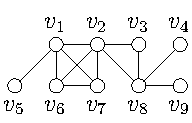
\includegraphics[height=1.6cm,bb=0 0 100 100]{examples/SecDomExa.pdf}} \hspace{0.5cm} \subfigure[]{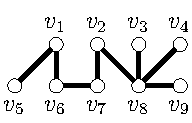
\includegraphics[height=1.6cm,bb=0 0 100 100]{examples/SecDomExa1.pdf}} \hspace{0.5cm} \subfigure[]{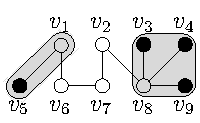
\includegraphics[height=1.6cm,bb=0 0 100 100]{examples/SecDomExb.pdf}} \hspace{0.5cm} \subfigure[]{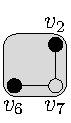
\includegraphics[height=1.6cm,bb=0 0 100 100]{examples/SecDomExc.pdf}} \end{center}

\vspace{-0.6cm}

\caption{(a) A graph $G_1$ for which $\gamma_s(G_1)=4$. (b) A spanning tree of $G_1$. (c)--(d) The result of identifying and pruning away end-clusters of the spanning tree in (b) according to Algorithm \ref{heuristic} to arrive at the secure dominating set $\{v_2,v_3,v_4,v_5,v_6,v_9\}$ of cardinality $6$ for $G_1$.} \label{treeboundpic} \end{figure}
Results are presented in Table~\ref{circulants} for all non-isomorphic, connected circulants of orders $n \leq 11$. 

\begin{table}[htb!]\centering\footnotesize
 \begin{tabular}{crrr|@{\hspace{0.1cm}}r@{\hspace{0.1cm}}r@{\hspace{0.3cm}}r@{\hspace{0.1cm}}r@{\hspace{0.1cm}}r@{\hspace{0.1cm}}|rrrr}\hline
	&		&		&		&		\multicolumn{5}{c|}{BR}					&	\multicolumn{4}{c}{BB}							\\
Graph	&	$n$	&	$|R|$	&	$\gamma_s$	&	&	Calls	&	&	Time	&	&	LB	&	UB	&	Calls	&	Time	\\\hline
${\cal{C}}_3\langle1\rangle$	&	3	&	1	&	1	&	&	\,3	&	&	0.01	&	&	1	&	1	&	\,3	&	0.01	\\\hline
${\cal{C}}_4\langle1\rangle$	&	4	&	0	&	2	&	&	\,21	&	&	0.01	&	&	2	&	2	&	\,21	&	0.01	\\
${\cal{C}}_4\langle1,2\rangle$	&	4	&	1	&	1	&	&	\,3	&	&	0.01	&	&	1	&	2	&	\,3	&	0.01	\\\hline
${\cal{C}}_5\langle1\rangle$	&	5	&	0	&	3	&	&	\,51	&	&	0.03	&	&	2	&	3	&	\,51	&	0.02	\\
${\cal{C}}_5\langle1,2\rangle$	&	5	&	1	&	1	&	&	\,3	&	&	0.01	&	&	1	&	1	&	\,3	&	0.01	\\\hline
${\cal{C}}_6\langle1\rangle$	&	6	&	0	&	3	&	&	\,95	&	&	0.04	&	&	2	&	3	&	\,83	&	0.04	\\
${\cal{C}}_6\langle1,2\rangle$	&	6	&	0	&	2	&	&	\,43	&	&	0.02	&	&	2	&	2	&	\,43	&	0.02	\\
${\cal{C}}_6\langle1,3\rangle$	&	6	&	0	&	3	&	&	\,85	&	&	0.04	&	&	2	&	3	&	\,83	&	0.04	\\
${\cal{C}}_6\langle2,3\rangle$	&	6	&	0	&	2	&	&	\,57	&	&	0.03	&	&	2	&	2	&	\,43	&	0.02	\\
${\cal{C}}_6\langle1,2,3\rangle$	&	6	&	1	&	1	&	&	\,3	&	&	0.01	&	&	1	&	1	&	\,3	&	0.01	\\\hline
${\cal{C}}_7\langle1\rangle$	&	7	&	0	&	3	&	&	\,199	&	&	0.09	&	&	3	&	3	&	\,149	&	0.07	\\
${\cal{C}}_7\langle1,2\rangle$	&	7	&	0	&	2	&	&	\,109	&	&	0.07	&	&	2	&	3	&	\,75	&	0.03	\\
${\cal{C}}_7\langle1,2,3\rangle$	&	7	&	1	&	1	&	&	\,3	&	&	0.01	&	&	1	&	1	&	\,3	&	0.01	\\\hline
${\cal{C}}_8\langle1\rangle$	&	8	&	0	&	4	&	&	\,411	&	&	0.21	&	&	3	&	4	&	\,285	&	0.17	\\
${\cal{C}}_8\langle1,2\rangle$	&	8	&	0	&	3	&	&	\,217	&	&	0.14	&	&	2	&	3	&	\,189	&	0.11	\\
${\cal{C}}_8\langle1,3\rangle$	&	8	&	0	&	4	&	&	\,345	&	&	0.16	&	&	2	&	4	&	\,319	&	0.24	\\
${\cal{C}}_8\langle1,4\rangle$	&	8	&	0	&	3	&	&	\,317	&	&	0.18	&	&	2	&	3	&	\,199	&	0.11	\\
${\cal{C}}_8\langle1,2,3\rangle$	&	8	&	0	&	2	&	&	\,73	&	&	0.05	&	&	2	&	2	&	\,73	&	0.03	\\
${\cal{C}}_8\langle1,2,4\rangle$	&	8	&	0	&	2	&	&	\,117	&	&	0.08	&	&	2	&	3	&	\,73	&	0.03	\\
${\cal{C}}_8\langle1,3,4\rangle$	&	8	&	0	&	2	&	&	\,87	&	&	0.06	&	&	2	&	2	&	\,73	&	0.03	\\
${\cal{C}}_8\langle1,2,3,4\rangle$	&	8	&	1	&	1	&	&	\,3	&	&	0.00	&	&	1	&	1	&	\,3	&	0.02	\\\hline
 \end{tabular}\vspace{-0.21cm}
\caption{Results obtained by means of the algorithm in BR and BB for all non-isomorphic, connected circulants of orders not exceeding $n = 8$. The columns labelled LB and UB contain the initial values of the global variables {\sf LowerBound} and  {\sf UpperBound} for the branch-and-bound algorithm. The column labelled $|R|$ contain the number of redundancy classes in each graph.} \label{circulants}
\end{table}

%%%%%%%%%%%%%%%%%%



\appto\bibfont{\footnotesize}
  \printbibliography


\end{document}